\documentclass[a4paper,12pt]{article}

\usepackage[portuguese]{babel}
\usepackage[utf8]{inputenc}
\usepackage[T1]{fontenc}
\usepackage{lmodern}
\usepackage{amsmath, amssymb}
\usepackage{graphicx}
\usepackage{hyperref}
\usepackage{booktabs}
\usepackage{listings}
\usepackage{array}
\usepackage{float}

\lstset{
  inputencoding=utf8,
  extendedchars=true,
  literate=
   {á}{{\'a}}1
   {à}{{\`a}}1
   {â}{{\^a}}1
   {ã}{{\~a}}1
   {é}{{\'e}}1
   {ê}{{\^e}}1
   {í}{{\'i}}1
   {ó}{{\'o}}1
   {ô}{{\^o}}1
   {õ}{{\~o}}1
   {ú}{{\'u}}1
   {ç}{{\c{c}}}1
   {Á}{{\'A}}1
   {À}{{\`A}}1
   {Â}{{\^A}}1
   {Ã}{{\~A}}1
   {É}{{\'E}}1
   {Ê}{{\^E}}1
   {Í}{{\'I}}1
   {Ó}{{\'O}}1
   {Ô}{{\^O}}1
   {Õ}{{\~O}}1
   {Ú}{{\'U}}1
   {Ç}{{\c{C}}}1
}

\begin{document}

\begin{titlepage}
    \centering
    \vfill
    {\Large \textbf{Universidade de São Paulo}}\\[1.5cm]
    {\Large SME0110 - Programação Matemática}\\[0.5cm]
    {\Huge \textbf{Projeto 1 - Alocação de Alunos Monitores}}\\[1.5cm]
    \vfill
    \begin{flushleft}
        \textbf{Integrantes do Grupo:}\\
        \vspace{0.5cm}
        \begin{tabular}{ll}
            Lucas Greff Meneses & 13671615 \\
            Gabriel Barbosa de Oliveira & 12543415 \\
            Henrique Souza Marques  & 11815722 \\
            João Pedro Matos de Deus & 12677492\\
            Carlos Filipe de Castro Lemos & 12542630 \\
        \end{tabular}
    \end{flushleft}
    \vfill
    {\large \today}
\end{titlepage}

\tableofcontents
\newpage

\section{Introdução}

A alocação eficiente de monitores nas disciplinas universitárias é um processo fundamental para garantir a qualidade do ensino e o suporte adequado aos estudantes. Monitores desempenham um papel crucial ao auxiliar professores, tirar dúvidas e contribuir para o aprofundamento do conteúdo ministrado em sala de aula.

No contexto atual, a atribuição de monitores às disciplinas enfrenta desafios relacionados à compatibilidade entre as preferências e qualificações dos monitores e as necessidades específicas de cada disciplina. Além disso, é importante considerar a equidade na distribuição das oportunidades entre os monitores candidatos.

Este projeto tem como objetivo desenvolver um modelo matemático para otimizar a alocação de monitores, maximizar a satisfação das preferências e qualificações dos monitores e atender às demandas das disciplinas. Para isso, implementamos o modelo em Python, utilizando o \textbf{algoritmo inteiro} aprendido em sala de aula, e exploramos uma abordagem alternativa por meio de um \textbf{algoritmo genético}.

Além do modelo matemático, desenvolvemos um software capaz de receber os dados dos monitores e realizar as alocações de forma automatizada. Este software oferece uma interface amigável e flexível, permitindo ajustar parâmetros e considerar diferentes cenários de alocação.

Todo o código, tanto dos algoritmos quanto do software, está disponível no \href{https://github.com/ethoshomo/scheduler-class-assistant}{repositório GitHub}.

Ao longo deste relatório, apresentamos a descrição detalhada do problema, o modelo matemático proposto, a implementação computacional realizada e os testes computacionais conduzidos. Também comparamos o desempenho do algoritmo inteiro com o algoritmo genético, analisando vantagens e limitações de cada abordagem.

Por fim, discutimos os resultados obtidos, destacando as contribuições do trabalho e apontando possíveis direções para trabalhos futuros.


\section{Objetivos}

O objetivo deste projeto é implementar o modelo matemático de alocação de monitores utilizando a linguagem Python e realizar os testes computacionais especificados, empregando tanto o algoritmo inteiro, conforme aprendido em sala de aula, quanto um algoritmo genético desenvolvido pelo grupo. Além disso, busca-se desenvolver um software capaz de receber um arquivo com os dados dos monitores e efetuar as alocações de forma otimizada, priorizando monitores com as maiores médias e maximizando o número de disciplinas atendidas, de modo a atender às necessidades do problema proposto e fornecer uma ferramenta prática para a gestão de monitores nas disciplinas.


\section{Descrição do Problema}

Este projeto aborda o problema de alocação de alunos monitores em disciplinas universitárias, onde um conjunto de monitores $A$ deve ser alocado a um conjunto de disciplinas $D$, levando em consideração as preferências e qualificações de cada monitor. Cada monitor, ao se inscrever, indica as disciplinas que está disposto a monitorar e apresenta uma pontuação correspondente à sua média ponderada acadêmica. O objetivo é maximizar a soma das pontuações dos monitores alocados, priorizando aqueles com as maiores médias, e simultaneamente maximizar o número de disciplinas atendidas. Para alcançar esse objetivo, é necessário formular um modelo matemático que considere as restrições de que cada disciplina pode ter no máximo um monitor, cada monitor pode ser alocado a no máximo uma disciplina, e um monitor só pode ser alocado a uma disciplina se tiver manifestado interesse em monitorá-la. A solução deste problema envolve a implementação computacional do modelo e a análise dos resultados obtidos a partir de diferentes testes computacionais.


\subsection{Parâmetros e Variáveis}

\begin{table}[h!]
    \centering
    \caption{Parâmetros e variáveis do modelo}
    \begin{tabular}{l p{10cm}}
        \toprule
        \textbf{Parâmetros} & \\
        $A$ & Conjunto de monitores, $a \in \{1, \dots, |A|\}$. \\
        $D$ & Conjunto de disciplinas, $d \in \{1, \dots, |D|\}$. \\
        $s_{ad}$ & 1 se o monitor $a$ está disposto a monitorar a disciplina $d$, 0 caso contrário. \\
        $N_a$ & Nota média do monitor $a$. \\
        \midrule
        \textbf{Variáveis} & \\
        $x_{ad}$ & 1 se o monitor $a$ é alocado para a disciplina $d$, 0 caso contrário. \\
        $y_d$ & 1 se a disciplina $d$ não possui monitor, 0 caso contrário. \\
        \bottomrule
    \end{tabular}
\end{table}

\subsection{Modelo Matemático}

\begin{align}
    \text{Maximizar} \quad & \sum_{d \in D} \sum_{a \in A} N_a \cdot x_{ad} - \sum_{d \in D} y_d \\
    \text{Sujeito a:} \quad & \sum_{a \in A} x_{ad} + y_d = 1, \quad \forall d \in D \\
    & \sum_{d \in D} x_{ad} \leq 1, \quad \forall a \in A \\
    & x_{ad} \leq s_{ad}, \quad \forall a \in A, \forall d \in D \\
    & x_{ad} \in \{0,1\}, \quad \forall a \in A, \forall d \in D \\
    & y_d \in \{0,1\}, \quad \forall d \in D
\end{align}

\section{Implementação}

O modelo matemático foi implementado em Python utilizando a biblioteca \textit{PuLP}, que é um framework para modelagem e resolução de problemas de otimização linear e inteira. O solver utilizado foi o \textit{CBC} (Coin-or Branch and Cut), um solver de programação inteira mista open-source integrado ao \textit{PuLP}. A implementação envolveu a definição das variáveis de decisão, da função objetivo e das restrições conforme o modelo proposto. Além disso, utilizamos recursos do Python para leitura dos dados dos monitores a partir de um arquivo Excel e para manipulação de estruturas de dados como listas e dicionários, o que facilitou a construção dinâmica do modelo de acordo com as entradas fornecidas.


\subsection{Desenvolvimento do Software}

O front-end foi construído utilizando JavaScript React, proporcionando uma interface dinâmica e responsiva para que os usuários interajam com o sistema de forma fluida. Para os algoritmos de otimização, incluindo tanto o modelo matemático quanto o algoritmo genético, utilizamos Python devido ao seu rico ecossistema de bibliotecas e ferramentas adequadas para tarefas computacionais complexas. Para conectar o front-end com o código de otimização, empregamos o Tauri, um framework moderno escrito em Rust. O Tauri permitiu uma comunicação eficiente e segura entre o front-end em JavaScript e o back-end em Python, melhorando o desempenho geral da aplicação. Além disso, realizamos o pré-processamento dos dados usando o Python Pandas, o que nos possibilitou manipular e organizar grandes conjuntos de dados de forma eficaz antes de serem inseridos nos modelos de otimização. Essa abordagem integrada, combinando React, Python, Rust e Pandas, facilitou o desenvolvimento de uma solução de software robusta e eficiente

\subsection{Algoritmo Branch-and-Cut}

O Branch-and-Cut funciona combinando os métodos de Branch-and-Bound e Cutting Planes. Inicialmente, ele resolve a relaxação linear do problema (ignorando as restrições de integralidade) usando o algoritmo Simplex. Se a solução obtida não satisfizer as restrições inteiras, o algoritmo gera cortes—restrições lineares adicionais que eliminam porções do espaço de solução que não contêm soluções inteiras viáveis. Em seguida, o algoritmo realiza a ramificação (branching), dividindo o problema original em subproblemas menores ao fixar valores para as variáveis inteiras fracionárias. Esses subproblemas são resolvidos recursivamente, aplicando novamente cortes e ramificação conforme necessário. O processo continua até que uma solução ótima inteira seja encontrada ou que todos os subproblemas tenham sido explorados, garantindo assim a otimização global dentro das restrições inteiras.

\subsection{Algoritmo Genético}

Um algoritmo evolucionário genético é uma técnica de otimização inspirada na evolução natural da biologia. Em outras palavras, trata-se de uma simulação do processo evolutivo em que uma determinada população de indivíduos é submetida a processos genéticos durante uma determinada quantidade de gerações. A principal ideia é que, a cada geração, todos os indivíduos da população estarão sujeitos a processos de acasalamento (\textit{mate}) e mutações (\textit{mutation}), bem como serão avaliados pela função objetivo (\textit{fitness}), sendo certo que apenas uma parte dos indivíduos que forem melhor avaliados será levada para a próxima geração em razão da seleção natural (\textit{select}).

No caso do trabalho, a solução do problema consistia em obter uma lista de alunos alocados como monitores para uma determinada turma, de acordo com critérios de maximização de salas atendidas por monitores e maximização dos interesses dos alunos escolhidos. Essa solução foi modelada para ser obtida por meio do algoritmo genético da biblioteca \textbf{DEAP}. Assim, modelamos a solução com os identificadores dos alunos em posição correspondente à lista de turmas das disciplinas. Por exemplo:

\subsection*{Turmas das Disciplinas}

\begin{table}[H]
    \centering
    \begin{tabular}{|c|c|c|c|c|c|c|}
        \hline
        Lab-T1 & Lab-T2 & Álgebra-T1 & Álgebra-T2 & \dots & Algoritmo-T3 \\
        \hline
    \end{tabular}
\end{table}

\subsection*{Indivíduo}

\begin{table}[H]
    \centering
    \begin{tabular}{|c|c|c|c|c|c|c|}
        \hline
        1 & 10 & 40 & 0 & \dots & 0 \\
        \hline
    \end{tabular}
\end{table}


Desse modo, o aluno cujo identificador é 1 foi alocado para a turma \textit{Lab-T1} (posição/index = 0), enquanto o aluno cujo identificador é 10 foi alocado para a turma \textit{Lab-T2} (posição 1) e assim sucessivamente. Caso a turma não tenha nenhum aluno alocado, em razão de não haver inscritos, a posição correspondente foi zerada, como aconteceu com \textit{Álgebra-T2} e \textit{Algoritmo-T3}.

No código da biblioteca, cada indivíduo (\textit{Individual}) é concebido como uma representação da solução final. Por isso, os modelos do indivíduo foram construídos como sendo uma lista de identificadores, a qual possui o atributo de aptidão atrelado (\textit{fitness}). Nesse contexto, a lista de identificadores é gerada pela função \texttt{create\_individual}, que segue as características descritas acima e usa critérios para eliminar a repetição de monitores em turmas diferentes, bem como emprega aleatoriedade para evitar vieses de escolha. Por sua vez, o atributo de aptidão é calculado pela função \texttt{evaluate\_individual} (\texttt{evaluate}). Essa função tem como objetivo calcular o grau de aptidão na alocação de monitores daquele indivíduo em específico por meio da distância euclidiana entre a quantidade de salas e o interesse do aluno.

Sobre o interesse do aluno, podemos entendê-lo como o simples somatório das notas ponderadas dos monitores ou podemos calcular o interesse de forma mais sofisticada, usando a nota ponderada e a preferência do aluno, de acordo com a seguinte fórmula:

\[
i = n \cdot e^{-0{,}4 \cdot (p - 1)},
\]

onde:
\begin{itemize}
    \item $i$ = interesse,
    \item $n$ = nota ponderada \quad $[0,10]$,
    \item $p$ = preferência \quad $\{1,2,3,4,5,6,\dots\}$ -- sendo maior o interesse quanto menor seu valor.
\end{itemize}

Sobre a avaliação, ainda é necessário explicar que a quantidade de salas precisa ser ajustada pela multiplicação pelo fator 10 (com a finalidade de evitar vieses em relação às notas).

Por sua vez, a população (\textit{population}) é gerada como uma lista de indivíduos, sendo certo que esses indivíduos irão passar por processos de evolução genética representados pelo acasalamento (\textit{mate}), mutações (\textit{mutate}) e seleção natural por elitismo (\textit{select}) a cada uma das gerações. Essas funções garantem a realização das recombinações genéticas para permitir que o algoritmo faça uma melhor exploração do espaço de busca. Vale ainda acrescentar que toda essa evolução é automatizada pela biblioteca \textbf{DEAP} por meio da função \texttt{algorithms.eaSimple}.

Por exemplo, o acasalamento é representativo do \textit{crossover}, o qual é automatizado pela função \texttt{tools.cxTwoPoint}, função que promove uma recombinação aleatória de dois indivíduos em um ponto de ruptura, da seguinte forma:

\begin{figure}[h!]
    \centering
    \includegraphics[width=0.8\textwidth]{crossing_over.png}
    \caption{Exemplo de crossing over}
    \label{fig:exemplo}
\end{figure}


As mutações servem para gerar aleatoriedade e não deixar o algoritmo convergir em mínimos locais. Por isso, utilizamos a função \texttt{mutate} para promover a troca aleatória de monitores constituintes do indivíduo - podendo, inclusive, repetir monitores (indivíduos não viáveis que serão eliminados na seleção).

Após a ocorrência desses processos, o algoritmo irá fazer uma avaliação dos indivíduos da população e promoverá uma seleção natural por elitismo (função \texttt{selection\_elitism}). Em outras palavras, apenas 20\% dos indivíduos mais adaptados, ou seja, mais bem avaliados, serão levados para a próxima geração, enquanto que os outros 80\% serão substituídos por novos indivíduos produzidos aleatoriamente pela função \texttt{create\_individual}.

Ao final, depois de todas as gerações, será retornado o melhor indivíduo encontrado no processo evolutivo.

\section{Testes Computacionais}

Nesta seção, estão os resultados dos testes computacionais exigidos no projeto para o \textbf{algoritmo Branch-and-Cut}.

\subsection{Teste 1}

O modelo foi executado com os dados do arquivo \verb|Dados_monitores.xlsx|, de acordo com as especificações.

\begin{lstlisting}[breaklines=true]
Solução Encontrada: 478.3
Status da solução: 1 1
Tempo de execução: 0.17 segundos

Monitores alocados:
Monitor 14590001 foi alocado para a disciplina 19.
Monitor 14580006 foi alocado para a disciplina 21.
Monitor 14570008 foi alocado para a disciplina 12.
Monitor 10270009 foi alocado para a disciplina 43.
Monitor 12540012 foi alocado para a disciplina 47.
Monitor 14560014 foi alocado para a disciplina 28.
Monitor 13690016 foi alocado para a disciplina 59.
Monitor 11210018 foi alocado para a disciplina 0.
Monitor 10690020 foi alocado para a disciplina 48.
Monitor 11800021 foi alocado para a disciplina 25.
Monitor 14550022 foi alocado para a disciplina 40.
Monitor 89570023 foi alocado para a disciplina 57.
Monitor 14560015 foi alocado para a disciplina 62.
Monitor 14710024 foi alocado para a disciplina 29.
Monitor 13870027 foi alocado para a disciplina 42.
Monitor 12540029 foi alocado para a disciplina 30.
Monitor 12620030 foi alocado para a disciplina 35.
Monitor 14590031 foi alocado para a disciplina 36.
Monitor 12550033 foi alocado para a disciplina 27.
Monitor 13670034 foi alocado para a disciplina 56.
Monitor 13670035 foi alocado para a disciplina 61.
Monitor 12540036 foi alocado para a disciplina 49.
Monitor 13680039 foi alocado para a disciplina 34.
Monitor 13690044 foi alocado para a disciplina 15.
Monitor 11910046 foi alocado para a disciplina 16.
Monitor 14610047 foi alocado para a disciplina 23.
Monitor 14560048 foi alocado para a disciplina 9.
Monitor 11790052 foi alocado para a disciplina 11.
Monitor 12550013 foi alocado para a disciplina 24.
Monitor 14600054 foi alocado para a disciplina 8.
Monitor 12550055 foi alocado para a disciplina 18.
Monitor 14600056 foi alocado para a disciplina 39.
Monitor 11810057 foi alocado para a disciplina 14.
Monitor 12540058 foi alocado para a disciplina 58.
Monitor 11800060 foi alocado para a disciplina 22.
Monitor 13670063 foi alocado para a disciplina 1.
Monitor 11910064 foi alocado para a disciplina 33.
Monitor 14650065 foi alocado para a disciplina 31.
Monitor 13830061 foi alocado para a disciplina 51.
Monitor 55630067 foi alocado para a disciplina 17.
Monitor 10310070 foi alocado para a disciplina 54.
Monitor 11840071 foi alocado para a disciplina 38.
Monitor 11790072 foi alocado para a disciplina 26.
Monitor 15110073 foi alocado para a disciplina 3.
Monitor 12680075 foi alocado para a disciplina 37.
Monitor 10740076 foi alocado para a disciplina 50.
Monitor 14570078 foi alocado para a disciplina 52.
Monitor 14560079 foi alocado para a disciplina 4.
Monitor 13680080 foi alocado para a disciplina 32.
Monitor 13680081 foi alocado para a disciplina 6.
Monitor 13830083 foi alocado para a disciplina 60.
Monitor 10330084 foi alocado para a disciplina 13.
Monitor 14560087 foi alocado para a disciplina 7.
Monitor 14570088 foi alocado para a disciplina 10.
Monitor 14610089 foi alocado para a disciplina 2.
Monitor 11220090 foi alocado para a disciplina 53.
Monitor 14750091 foi alocado para a disciplina 41.
Monitor 12670095 foi alocado para a disciplina 5.
Monitor 12540096 foi alocado para a disciplina 55.

Monitores não alocados:
Monitor 11780000 NÃO foi alocado. Inscrito para as disciplinas: [38, 39, 40]
Monitor 12730002 NÃO foi alocado. Inscrito para as disciplinas: [41, 56, 57]
Monitor 14740004 NÃO foi alocado. Inscrito para as disciplinas: [5, 39]
Monitor 12680005 NÃO foi alocado. Inscrito para as disciplinas: [38, 39, 40, 56]
Monitor 10740003 NÃO foi alocado. Inscrito para as disciplinas: [38, 39, 40, 41, 42, 55, 56, 57]
Monitor 77770010 NÃO foi alocado. Inscrito para as disciplinas: [38, 39, 40, 41, 55, 56]
Monitor 14550011 NÃO foi alocado. Inscrito para as disciplinas: [56]
Monitor 13740007 NÃO foi alocado. Inscrito para as disciplinas: [27]
Monitor 11910017 NÃO foi alocado. Inscrito para as disciplinas: [27]
Monitor 13860019 NÃO foi alocado. Inscrito para as disciplinas: [6, 8, 9, 12, 62]
Monitor 11220025 NÃO foi alocado. Inscrito para as disciplinas: [14]
Monitor 12550032 NÃO foi alocado. Inscrito para as disciplinas: [23, 27]
Monitor 10770037 NÃO foi alocado. Inscrito para as disciplinas: [5]
Monitor 15500038 NÃO foi alocado. Inscrito para as disciplinas: [2, 11, 24]
Monitor 90390040 NÃO foi alocado. Inscrito para as disciplinas: [57, 58, 59, 60]
Monitor 13680041 NÃO foi alocado. Inscrito para as disciplinas: [7]
Monitor 12920042 NÃO foi alocado. Inscrito para as disciplinas: [41, 55]
Monitor 11890043 NÃO foi alocado. Inscrito para as disciplinas: [58]
Monitor 12670045 NÃO foi alocado. Inscrito para as disciplinas: [40, 41, 48]
Monitor 12550049 NÃO foi alocado. Inscrito para as disciplinas: [17]
Monitor 14610050 NÃO foi alocado. Inscrito para as disciplinas: [0, 7, 16]
Monitor 14560051 NÃO foi alocado. Inscrito para as disciplinas: [0, 1, 2, 3, 6, 7, 8, 9, 10, 11, 12]
Monitor 10720053 NÃO foi alocado. Inscrito para as disciplinas: [49]
Monitor 12710059 NÃO foi alocado. Inscrito para as disciplinas: [16]
Monitor 13270062 NÃO foi alocado. Inscrito para as disciplinas: [50]
Monitor 13730028 NÃO foi alocado. Inscrito para as disciplinas: [36, 55]
Monitor 11910066 NÃO foi alocado. Inscrito para as disciplinas: [38, 39, 40, 54, 55, 56]
Monitor 11210068 NÃO foi alocado. Inscrito para as disciplinas: [32]
Monitor 94220069 NÃO foi alocado. Inscrito para as disciplinas: [8, 30, 36]
Monitor 14560074 NÃO foi alocado. Inscrito para as disciplinas: [39, 40]
Monitor 13820077 NÃO foi alocado. Inscrito para as disciplinas: [40]
Monitor 53400026 NÃO foi alocado. Inscrito para as disciplinas: [23, 24]
Monitor 14650082 NÃO foi alocado. Inscrito para as disciplinas: [24]
Monitor 13710085 NÃO foi alocado. Inscrito para as disciplinas: [41, 55]
Monitor 15490086 NÃO foi alocado. Inscrito para as disciplinas: [0, 2, 7, 11]
Monitor 13670092 NÃO foi alocado. Inscrito para as disciplinas: [1, 3, 22]
Monitor 14140093 NÃO foi alocado. Inscrito para as disciplinas: [17, 18]
Monitor 11870094 NÃO foi alocado. Inscrito para as disciplinas: [38, 39, 40, 52, 54, 56]

Disciplinas não atendidas e seus inscritos:
A disciplina 20 não foi atendida por nenhum monitor. Inscritos: [14590001, 14580006, 10270009, 12540012, 12620030]
A disciplina 44 não foi atendida por nenhum monitor. Inscritos: [10270009]
A disciplina 45 não foi atendida por nenhum monitor. Inscritos: [10270009]
A disciplina 46 não foi atendida por nenhum monitor. Inscritos: [12540012]
\end{lstlisting}

É possível perceber que apenas 4 disciplinas não foram atendidas pelo modelo. Todos os inscritos que não receberam monitorias não se inscreveram nas disciplinas que ficaram sem monitores.

\subsection{Teste 2}

No caso de haver disciplinas sem monitores e inscritos que já cursaram essas disciplinas, seria interessante, no ponto de vista de um gestor, sugerir a esses inscritos a opção de monitorar as disciplinas sem monitores.

\subsection{Teste 3}

Os alunos selecionados e as respectivas disciplinas atribuídas foram: 11780000, 13870027, 12550032, 12550033 e 13690044; e 20, 44, 45, 46, 18. O resultado do modelo foi:

\begin{lstlisting}[breaklines=true]
Solução Encontrada: 511.00000000000006
Status da solução: 1 1
Tempo de execução: 0.19 segundos

Monitores alocados:
Monitor 11780000 foi alocado para a disciplina 20.
Monitor 14590001 foi alocado para a disciplina 19.
Monitor 14580006 foi alocado para a disciplina 21.
Monitor 10740003 foi alocado para a disciplina 42.
Monitor 14570008 foi alocado para a disciplina 12.
Monitor 10270009 foi alocado para a disciplina 43.
Monitor 12540012 foi alocado para a disciplina 47.
Monitor 13740007 foi alocado para a disciplina 27.
Monitor 14560014 foi alocado para a disciplina 28.
Monitor 13690016 foi alocado para a disciplina 59.
Monitor 11210018 foi alocado para a disciplina 0.
Monitor 10690020 foi alocado para a disciplina 48.
Monitor 11800021 foi alocado para a disciplina 25.
Monitor 14550022 foi alocado para a disciplina 40.
Monitor 89570023 foi alocado para a disciplina 57.
Monitor 14560015 foi alocado para a disciplina 62.
Monitor 14710024 foi alocado para a disciplina 29.
Monitor 13870027 foi alocado para a disciplina 44.
Monitor 12540029 foi alocado para a disciplina 30.
Monitor 12620030 foi alocado para a disciplina 35.
Monitor 14590031 foi alocado para a disciplina 36.
Monitor 12550032 foi alocado para a disciplina 45.
Monitor 12550033 foi alocado para a disciplina 46.
Monitor 13670034 foi alocado para a disciplina 55.
Monitor 13670035 foi alocado para a disciplina 61.
Monitor 12540036 foi alocado para a disciplina 49.
Monitor 13680039 foi alocado para a disciplina 34.
Monitor 13690044 foi alocado para a disciplina 15.
Monitor 11910046 foi alocado para a disciplina 16.
Monitor 14610047 foi alocado para a disciplina 23.
Monitor 14560048 foi alocado para a disciplina 2.
Monitor 11790052 foi alocado para a disciplina 11.
Monitor 12550013 foi alocado para a disciplina 24.
Monitor 14600054 foi alocado para a disciplina 6.
Monitor 12550055 foi alocado para a disciplina 18.
Monitor 14600056 foi alocado para a disciplina 38.
Monitor 11810057 foi alocado para a disciplina 14.
Monitor 12540058 foi alocado para a disciplina 58.
Monitor 11800060 foi alocado para a disciplina 22.
Monitor 13670063 foi alocado para a disciplina 1.
Monitor 11910064 foi alocado para a disciplina 33.
Monitor 14650065 foi alocado para a disciplina 31.
Monitor 13830061 foi alocado para a disciplina 51.
Monitor 55630067 foi alocado para a disciplina 17.
Monitor 10310070 foi alocado para a disciplina 39.
Monitor 11840071 foi alocado para a disciplina 56.
Monitor 11790072 foi alocado para a disciplina 26.
Monitor 15110073 foi alocado para a disciplina 3.
Monitor 12680075 foi alocado para a disciplina 37.
Monitor 10740076 foi alocado para a disciplina 50.
Monitor 14570078 foi alocado para a disciplina 52.
Monitor 14560079 foi alocado para a disciplina 4.
Monitor 13680080 foi alocado para a disciplina 32.
Monitor 13680081 foi alocado para a disciplina 7.
Monitor 13830083 foi alocado para a disciplina 54.
Monitor 10330084 foi alocado para a disciplina 13.
Monitor 14560087 foi alocado para a disciplina 9.
Monitor 14570088 foi alocado para a disciplina 8.
Monitor 14610089 foi alocado para a disciplina 10.
Monitor 11220090 foi alocado para a disciplina 53.
Monitor 14750091 foi alocado para a disciplina 41.
Monitor 12670095 foi alocado para a disciplina 5.
Monitor 12540096 foi alocado para a disciplina 60.

Monitores não alocados:
Monitor 12730002 NÃO foi alocado. Inscrito para as disciplinas: [41, 56, 57]
Monitor 14740004 NÃO foi alocado. Inscrito para as disciplinas: [5, 39]
Monitor 12680005 NÃO foi alocado. Inscrito para as disciplinas: [38, 39, 40, 56]
Monitor 77770010 NÃO foi alocado. Inscrito para as disciplinas: [38, 39, 40, 41, 55, 56]
Monitor 14550011 NÃO foi alocado. Inscrito para as disciplinas: [56]
Monitor 11910017 NÃO foi alocado. Inscrito para as disciplinas: [27]
Monitor 13860019 NÃO foi alocado. Inscrito para as disciplinas: [6, 8, 9, 12, 62]
Monitor 11220025 NÃO foi alocado. Inscrito para as disciplinas: [14]
Monitor 10770037 NÃO foi alocado. Inscrito para as disciplinas: [5]
Monitor 15500038 NÃO foi alocado. Inscrito para as disciplinas: [2, 11, 24]
Monitor 90390040 NÃO foi alocado. Inscrito para as disciplinas: [57, 58, 59, 60]
Monitor 13680041 NÃO foi alocado. Inscrito para as disciplinas: [7]
Monitor 12920042 NÃO foi alocado. Inscrito para as disciplinas: [41, 55]
Monitor 11890043 NÃO foi alocado. Inscrito para as disciplinas: [58]
Monitor 12670045 NÃO foi alocado. Inscrito para as disciplinas: [40, 41, 48]
Monitor 12550049 NÃO foi alocado. Inscrito para as disciplinas: [17]
Monitor 14610050 NÃO foi alocado. Inscrito para as disciplinas: [0, 7, 16]
Monitor 14560051 NÃO foi alocado. Inscrito para as disciplinas: [0, 1, 2, 3, 6, 7, 8, 9, 10, 11, 12]
Monitor 10720053 NÃO foi alocado. Inscrito para as disciplinas: [49]
Monitor 12710059 NÃO foi alocado. Inscrito para as disciplinas: [16]
Monitor 13270062 NÃO foi alocado. Inscrito para as disciplinas: [50]
Monitor 13730028 NÃO foi alocado. Inscrito para as disciplinas: [36, 55]
Monitor 11910066 NÃO foi alocado. Inscrito para as disciplinas: [38, 39, 40, 54, 55, 56]
Monitor 11210068 NÃO foi alocado. Inscrito para as disciplinas: [32]
Monitor 94220069 NÃO foi alocado. Inscrito para as disciplinas: [8, 30, 36]
Monitor 14560074 NÃO foi alocado. Inscrito para as disciplinas: [39, 40]
Monitor 13820077 NÃO foi alocado. Inscrito para as disciplinas: [40]
Monitor 53400026 NÃO foi alocado. Inscrito para as disciplinas: [23, 24]
Monitor 14650082 NÃO foi alocado. Inscrito para as disciplinas: [24]
Monitor 13710085 NÃO foi alocado. Inscrito para as disciplinas: [41, 55]
Monitor 15490086 NÃO foi alocado. Inscrito para as disciplinas: [0, 2, 7, 11]
Monitor 13670092 NÃO foi alocado. Inscrito para as disciplinas: [1, 3, 22]
Monitor 14140093 NÃO foi alocado. Inscrito para as disciplinas: [17, 18]
Monitor 11870094 NÃO foi alocado. Inscrito para as disciplinas: [38, 39, 40, 52, 54, 56]

Disciplinas não atendidas e seus inscritos:
\end{lstlisting}

Como as disciplinas adicionadas foram aquelas que ficaram sem monitores, todas disciplinas receberam monitores e o valor da função objetivo mudou de 478 para 511, mostrando que o algoritmo chegou em uma solução melhor.

\subsection{Teste 4}

\begin{table}[h!]
    \centering
    \begin{tabular}{|c|c|c|c|}
        \hline
        \textbf{Fator de Escala} & \textbf{Tempo de Execução (s)} & \textbf{Valor do Objetivo} & \textbf{Gap (\%)} \\
        \hline
        2 & 1.32 & 852.34 & 0.0 \\
        3 & 2.70 & 1353.17 & 0.0 \\
        5 & 7.06 & 2287.99 & 0.0 \\
        10 & 29.23 & 4623.08 & 0.0 \\
        15 & 79.06 & 6601.22 & 0.0 \\
        \hline
    \end{tabular}
    \caption{Resultados das instâncias geradas com diferentes fatores de escala}
    \label{tab:resultados}
\end{table}

É possível perceber na Tabela 2 que, com o aumento dos dados, o tempo de execução aumentou. Além disso, como o gap é 0 em todas as instâncias, é possível concluir que o algoritmo alcançou o valor ótimo em todos os casos.

\subsection{Teste 5}

\begin{table}[h!]
    \centering
    \begin{tabular}{|c|c|c|c|}
        \hline
        \textbf{Fator de Escala} & \textbf{Tempo de Execução (s)} & \textbf{Valor do Objetivo} & \textbf{Gap (\%)} \\
        \hline
        2 & 1.19 & 852.34 & 0.0 \\
        3 & 2.63 & 1353.17 & 0.0 \\
        5 & 7.37 & 2287.99 & 0.0 \\
        10 & 29.05 & 4623.08 & 0.0 \\
        15 & 79.02 & 6601.22 & 0.0 \\
        \hline
    \end{tabular}
    \caption{Resultados das instâncias geradas com diferentes fatores de escala}
    \label{tab:resultados}
\end{table}

É possível perceber na Tabela 3 que, mesmo com a opção "cuts" desativada, não houve alterações significativas em nenhum aspecto. 

\subsection{Teste 6}

\begin{table}[h!]
    \centering
    \begin{tabular}{|c|c|c|c|}
        \hline
        \textbf{Fator de Escala} & \textbf{Tempo de Execução (s)} & \textbf{Valor do Objetivo} & \textbf{Gap (\%)} \\
        \hline
        2 & 1.20 & 852.34 & 0.0 \\
        3 & 2.56 & 1353.17 & 0.0 \\
        5 & 7.02 & 2287.99 & 0.0 \\
        10 & 29.31 & 4623.08 & 0.0 \\
        15 & 78.88 & 6601.22 & 0.0 \\
        \hline
    \end{tabular}
    \caption{Resultados das instâncias geradas com diferentes fatores de escala}
    \label{tab:resultados}
\end{table}

É possível perceber na Tabela 4 que, mesmo com a opção "presolve" desativada, não houve alterações significativas em nenhum aspecto.

\subsection{Teste 7}

As prioridades dos alunos foram incluídas na função objetivo como valores que refletem a preferência dos monitores por disciplinas. A prioridade ajustada (`prioridade\_adj`) é calculada invertendo as prioridades, de forma que um valor maior na prioridade resulte em um valor menor na função objetivo, garantindo que prioridades mais altas tenham maior impacto na maximização. A função objetivo maximiza uma combinação da nota acadêmica do aluno (Na[a]) e da prioridade ajustada, garantindo que os monitores sejam alocados às disciplinas que mais desejam, considerando também seu desempenho acadêmico.

As prioridades dos alunos foram incluídas na função objetivo como valores que refletem a preferência dos monitores por disciplinas. A prioridade ajustada (`prioridade\_adj`) é calculada invertendo as prioridades, de forma que um valor maior na prioridade resulte em um valor menor na função objetivo, garantindo que prioridades mais altas tenham maior impacto na maximização. A função objetivo maximiza uma combinação da nota acadêmica do aluno (`Na[a]`) e da prioridade ajustada, garantindo que os monitores sejam alocados às disciplinas que mais desejam, considerando também seu desempenho acadêmico.


\begin{table}[h!]
    \centering
    \begin{tabular}{|c|c|c|c|}
        \hline
        \textbf{Fator de Escala} & \textbf{Tempo de Execução (s)} & \textbf{Valor do Objetivo} & \textbf{Gap (\%)} \\
        \hline
        2 & 1.25 & 914610.90 & 0.0 \\
        3 & 2.57 & 1395544.12 & 0.0 \\
        5 & 7.00 & 2326132.93 & 0.0 \\
        10 & 29.71 & 4651309.27 & 0.0 \\
        15 & 82.79 & 6639543.43 & 0.0 \\
        \hline
    \end{tabular}
    \caption{Resultados das instâncias geradas com diferentes fatores de escala}
    \label{tab:resultados}
\end{table}

É possível perceber na Tabela 5 que, ao incluir no modelo as prioridades dos alunos, houve um ligeiro aumento no tempo de execução e um aumento significativo no valor da função objetivo.

\section{Análise Comparativa entre os Algoritmos}

Na figura 2, as salas atendidas por diferentes escalas da função \texttt{aumentar\_dados} estão postas para os dois algoritmos. É possível perceber que o algoritmo genético se aproxima bem do algoritmo inteiro, que sempre atinge o valor ótimo, mesmo em escalas muito grandes de dados. Já na figura 3, que expõe o tempo de execução dos algoritmos para diferentes escalas de dados, é possível perceber que o aalgoritmo genético leva muito mais tempo para encontrar uma solução. Isso se dá porque o algoritmo genético realiza uma busca heurística no espaço de soluções, o que envolve a criação e evolução de uma população de indivíduos ao longo de diversas gerações. Esse processo inclui operações como seleção, cruzamento (crossover) e mutação, que são computacionalmente intensivas. Além disso, a avaliação da aptidão de cada indivíduo na população em cada geração também consome tempo, especialmente em problemas com grandes escalas, onde o espaço de busca é maior e mais complexo.

\begin{figure}[H]
    \centering
    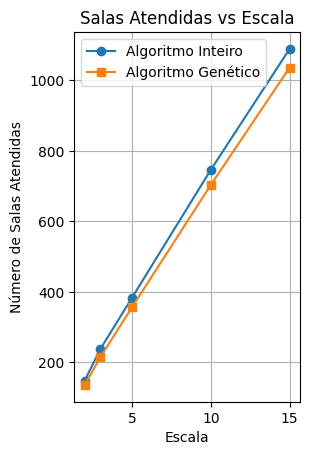
\includegraphics[width=0.6\textwidth]{salas_escala.png}
    \caption{Salas atendidas por escalas}
    \label{fig:salas_escala}
\end{figure}

\begin{figure}[H]
    \centering
    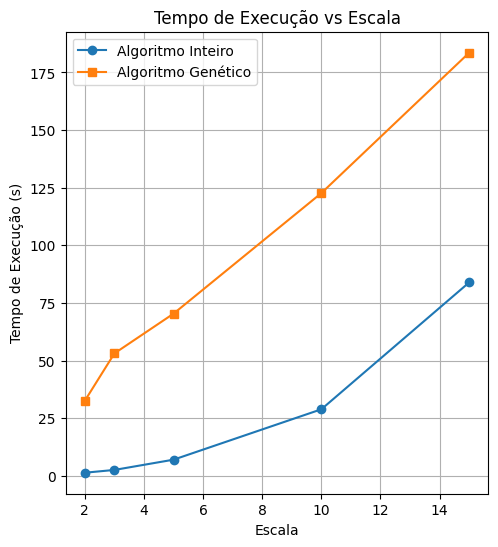
\includegraphics[width=0.6\textwidth]{tempo_escala.png}
    \caption{Tempo de execução por escalas}
    \label{fig:tempo_escala}
\end{figure}

\section{Atuação dos Integrantes}

\begin{itemize}
    \item \textbf{Lucas Greff Meneses:} desenvolveu o algoritmo inteiro de acordo com as especificações do trabalho e elaborou o relatório.

    \item \textbf{João Pedro Matos de Deus:} elaborou o arquivo \texttt{README.md} do repositório.

    \item \textbf{Henrique Souza Marques:} fez o processamento de dados e ajudou na integração entre front e backend.

    \item \textbf{Carlos Filipe de Castro Lemos:} desenvolveu o algoritmo genético e ajudou no processamento de dados.

    \item \textbf{Gabriel Barbosa de Oliveira:} desenvolveu o frontend do software e ajudou na integração entre front e backend.
\end{itemize}

\end{document}
